\documentclass[12pt, openany]{report}
\usepackage[utf8]{inputenc}
\usepackage[T1]{fontenc}
\usepackage[french]{babel}
\usepackage{xcolor}
\usepackage{amsmath}
\usepackage[colorinlistoftodos]{todonotes}
\usepackage[colorlinks=true, allcolors=black]{hyperref}
\usepackage[a4paper,left=2cm,right=2cm,top=2cm,bottom=2cm]{geometry}
\usepackage{verbatim}
\usepackage{listings}
\usepackage{hyperref}
\usepackage{boxedminipage}
\usepackage{pgfgantt}
\usepackage{float}
\usepackage{pdfpages}
\usetikzlibrary{babel}
\usepackage{varioref}
\usepackage{listingsutf8}
\usepackage{algorithm2e}
\usepackage{libertine}

\bibliographystyle{alpha}


\setlength{\parindent}{0cm}
\setlength{\parskip}{1ex plus 0.5ex minus 0.2ex}
\newcommand{\hsp}{\hspace{20pt}}
\newcommand{\HRule}{\rule{\linewidth}{0.5mm}}

\renewcommand{\thesection}{\arabic{section}}

\begin{document}

\begin{titlepage}
  \begin{sffamily}
  \begin{center}

    \textsc{\LARGE Projet de programmation}\\[0.3cm]
    
    
\includegraphics[scale=0.35]{images/img2.jpg}~\\[0.8cm]

    % Title
    \HRule \\[0.4cm]
    { \huge \bfseries Génération de playlistes musicales pour un groupe d’utilisateurs\\[0.4cm] }
    
    \HRule \\[1.5cm]
    
\includegraphics[scale=0.4]{images/img1.png}
    \\[1.5cm]

    % Authors and supervisors
    \begin{minipage}{0.4\textwidth}
      \begin{flushleft} \large
        Legendre \textsc{Alexandre}\\
        Chauveau \textsc{Amandine}\\
        Berardet \textsc{Titouan}\\
        Chen \textsc{Zhong Yi}\\
        Martin--Delozanne \textsc{Delphine}\\
      \end{flushleft}
    \end{minipage}
    \begin{minipage}{0.4\textwidth}
      \begin{flushright} \large
        \emph{Responsable de l'UE : } M. \textsc{Philippe Narbel}\\
        \emph{Client : } M. \textsc{Pierre Hanna}\\
        \emph{Chargé de TD : } M. \textsc{Philippe Narbel}
      \end{flushright}
    \end{minipage}

    \vfill

    % Bottom of the page
    {\large Version 1 : Janvier 2020 — Avril 2020}

  \end{center}
  \end{sffamily}
\end{titlepage}

\tableofcontents
\newpage

\section{Introduction}

\paragraph{}Actuellement, tout utilisateur d'un service de streaming de musique, comme Spotify ou Deezer par exemple, peut se voir recommander des playlists en fonction de ses propres goûts musicaux.
Cependant, il arrive que plusieurs personnes veuillent écouter de la musique ensemble au même endroit.
\paragraph{}Dans cette situation, le plus courant est qu'une personne du groupe impose sa playlist aux autres.
Afin de changer la tendance pour que l'ensemble du groupe soit satisfait par les musiques diffusées, nous proposons une application mobile qui créera une playlist associant les goûts musicaux de tous les utilisateurs.
\paragraph{}Par la connexion de plusieurs utilisateurs à une plateforme de streaming sur un même téléphone, notre application récupérera les informations publiques de ces utilisateurs pour former une liste de musiques combinant les goûts musicaux de toutes les personnes connectées. Différents algorithmes permettront la génération de cette playlist globale qui sera ensuite écoutée directement sur l'application.

\section{Description et analyse de l'existant}

\subsection{Flytrap : recommandation intelligente de musique pour un groupe}

\paragraph{}Flytrap \cite {Flytrap} est un environnement musical qui se base sur les goûts de ses utilisateurs afin de  créer automatiquement une bande sonore qui peut plaire à toutes les personnes présentes dans une même pièce. Pour ce faire Flytrap regarde quelles sont les musiques que les utilisateurs écoutent et enregistre les pistes ainsi que des informations sur la musique dans une base de données. Le système utilise ensuite ces données et les combine avec la connaissance de la façon dont les genres de musique interagissent  entre eux pour prendre des décisions sur ce qu’un groupe d’utilisateurs pourrait vouloir écouter. \\
Afin de décider quelles pistes ajouter à une playlist, le système utilise un mécanisme de vote par lequel un «agent» représentant chaque utilisateur présent dans la salle donne un vote numérique à chaque piste dans la base de données du système. Si l’utilisateur a déjà écouté une musique de l’artiste ou si le genre est similaire à la musique qu’il écoute habituellement, la chanson reçoit un score élevé. Les musiques obtenant des scores plus élevés ont ainsi une plus forte probabilité d’être jouées. De plus, le système dispose également d’un agent de DJ qui priorise le résultat du vote de l’utilisateur en fonction de certaines règles : ne pas jouer deux musiques d’affilées du même artiste et maintenir une cohérence entre les genres. Flytrap gère donc intelligemment la musique dans un espace peuplé de gens aux goûts disparates en permettant de découvrir de nouvelles musiques d’artistes jamais écoutés mais ayant des qualités similaires aux musiques aimées par les utilisateurs.

\subsection{MusicFX}

\paragraph{}MusicFX \cite {MusicFX} est un système de recommandation musicale qui permet aux membres d’un centre de fitness travaillant au même moment, d’influencer sans contrôler la musique diffusée.
\\
Pour ce faire, le système se base sur un algorithme qui prend en entrée un tableau représentant les préférences des utilisateurs présents dans la salle en fonction de genres musicaux. Ces valeurs vont de -2 (l’utilisateur déteste ce genre de musiques) à 2 (l’utilisateur adore ce genre de musiques). Une formule convertit alors toutes les préférences individuelles en des nombres non négatifs afin de pouvoir appliquer un opérateur de sélection aléatoire pondéré. Ces valeurs sont ensuite mises au carré afin d’élargir l’écart des probabilités de sélection entre les catégories les plus populaires et les catégories moins populaires. 
\\
Une fois la valeur de préférence de groupe calculée pour chacune des catégories, la liste des valeurs est triée par ordre décroissant, afin que la catégorie la plus populaire soit la première et la moins populaire soit la dernière. Comme la plupart des gens s’entraînent à la même heure et n’ont pas forcément envie d’écouter la même musique à chaque fois, le système utilise une politique de sélection de l’un des ‘m’ genres préférés (où m est défini dans le système).

\section{Outils}

\subsection{Interfaces de programmation}

\paragraph{}Les API de Spotify \cite{APISpotify} et Deezer \cite{APIDeezer} permettent de développer une application mobile tout en ayant accès à leurs données respectives. Ces données sont récupérables dès l'authentification d'un utilisateur (récupération de son ID Spotify ou Deezer). Elles se retrouvent ensuite, grâce aux requêtes utilisant l'ID, sous forme de classes, de méthodes, de fonctions et de constantes qui servent de "façade" par laquelle Spotify et Deezer offrent leurs services à d'autres logiciels. Par exemple, si l'on veut récupérer une chanson d'une playlist d'un utilisateur, les deux API sont capables de nous renvoyer la playlist correspondante avec les morceaux qu'elle contient, ainsi que des informations supplémentaires. De plus les API permettent également de récupérer des métadonnées
sur les artistes, les albums et morceaux de musique, directement à partir de leur catalogue de données.
\\
Elles proposent deux méthodes d'authentification :
\\- Par l'application Spotify/Deezer installée sur l'appareil de l'utilisateur.
\\- Par le navigateur Web.

\subsection{Algorithmes}

\paragraph{}Il existe différents algorithmes pour la recommandation de données pour un groupe d'utilisateurs. Pour un nombre d'utilisateurs et un nombre d'items fixés, chaque utilisateur a attribué une note à chaque item \cite {Group}. Ces algorithmes seront utilisés par notre application. Les items seront les artistes des musiques écoutées par les utilisateurs. Nous générerons les notes des items pour chaque utilisateur en fonction du nombre d'apparition de l'artiste dans ses playlists.
\\
\begin{itemize}
\item[1)] \textbf{Additive utilitarian strategy} : les notes pour chaque item sont additionnées. A partir de toutes les notes, il est possible d'obtenir un classement des différents items. Les items ayant obtenus des notes élevées sont considérés comme appréciés et sont donc en haut du classement. Il existe également une version de cette stratégie où les notes sont multipliées et non pas additionnées. L'avantage de cette stratégie est qu'elle est simple à comprendre et à implémenter. L'inconvénient est qu'elle est trop générique. Dans l'exemple ci-dessous, l'item i1 obtient un score correct et pourrait donc, dans le cadre de notre application, être intégré à la playlist alors que l'utilisateur u2 sera très insatisfait.
\\
\\
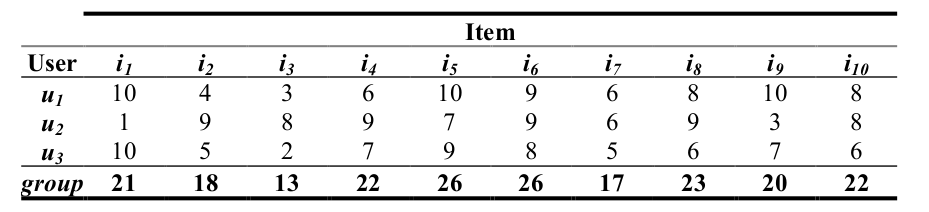
\includegraphics[scale=0.4]{images/_additive.png}

\textbf{Figure 1} : Sélection avec la stratégie d'addition. La liste ordonnée est : i5-i6,i8,i4-i10,i1,i9,i2,i7,i3.
\\
\item[2)] \textbf{Average without misery strategy} : chaque item reçoit une note moyenne en fonction des notes données par les utilisateurs. Les items ayant reçus une note en dessous d'un certain seuil par au moins un utilisateur ne sont pas considérés pour la suite. L'avantage de cette stratégie est qu'elle règle le problème soulevé par la stratégie précédente car le seuil, qui est fixé à 4 dans l'exemple ci-dessous, permet d'éviter qu'un utilisateur soit complètement insatisfait du choix d'un item.
\\
\\
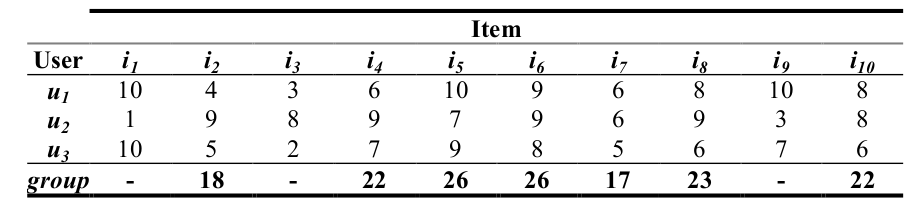
\includegraphics[scale=0.4]{images/_average_without_misery.png}

\textbf{Figure 2} : Sélection avec la stratégie de moyenne "sans misère". Le seuil ici est de 4. La liste ordonnée est : i5-i6,i8,i4-i10,i2,i7.
\\
\item[3)] \textbf{Borda count strategy} : les notes données par chaque utilisateur pour tous les items sont modifiées. Pour un utilisateur, l'item ayant reçu la moins bonne note reçoit une nouvelle note de 0. Les notes augmentent ensuite de 1 pour les items suivant. Les items ayant la même note initiale reçoivent tous la moyenne des nouvelles notes qui auraient du leur être attribuées. Par exemple, si deux items ont la même note et devraient recevoir les notes 2 et 3, ils reçoivent tous les deux la moyenne qui est de 2.5. Les nouvelles notes sont ensuite additionnées pour établir le classement. L'avantage de cette stratégie est qu'elle apporte de l'homogénéité à l'attribution des notes.
\\
\\
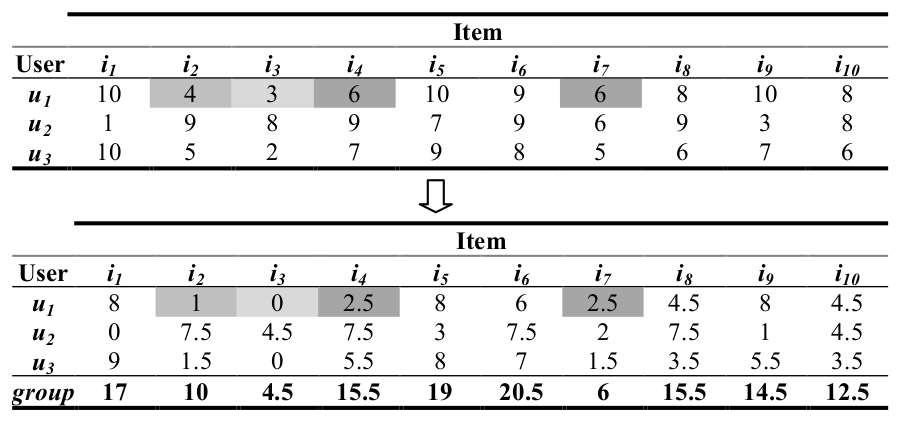
\includegraphics[scale=0.4]{images/_borda_count.png}

\textbf{Figure 3} : Sélection avec la stratégie borda count. La liste ordonnée est : i6, i5, i1, i4-i8, i9, i10, i2, i7, i3.
\end{itemize}

\newpage
\section{Description des besoins}

\subsection{Besoins fonctionnels}

Voici la liste non-exhaustive des différents besoins fonctionnels de l'application.

\begin{itemize}
\item[1) -] L'application doit \textbf{assurer les fonctions de lecture de base} : lecture et pause des playlists générées par nos algorithmes, ainsi que la possibilité de passer des titres musicaux. L'utilisateur devra avoir accès rapidement à une page sur l'application assurant ces fonctions. Notre application utilisera le media player de la plateforme choisie par l'utilisateur pour se connecter (voir besoin 4) ). Il faudra donc que cette plateforme (Spotify ou Deezer par exemple) soit installée sur le téléphone utilisé. Pendant la lecture des musiques, un utilisateur pourra indiquer à l'aide de boutons "j'aime" ou "je n'aime pas" s'il apprécie ou non une musique. Un panneau s'affichera alors pour indiquer à l'application quel utilisateur a fait l'action parmi les personnes connectées. L'application pourra également afficher la playlist courante pour que les utilisateurs voient les titres suivants.
\\
\item[2) -] L'application doit être en mesure de pouvoir \textbf{proposer une ou plusieurs playlists adaptées aux goûts des utilisateurs}, grâce aux informations recueillies sur la plateforme de streaming musicale choisie. 
Pour ce faire, l'application va se baser sur différents algorithmes de génération de playlists, reflétant les stratégies trouvées au sein d'une des ressources à disposition du projet \cite{Algorithme}. Nous implémenterons en priorité les stratégies présentées dans la section "3.2 Algorithmes" de ce document, à savoir : additive utilitarian strategy, average without misery et borda count.
\\
\item[3) -] L'application doit pouvoir \textbf{accéder aux informations sur la plateforme de streaming musicale pour chaque utilisateur} grâce à son API. L'utilisateur doit donc pour cela autoriser l'application à accéder à ses informations stockées sur la plateforme choisie. Ces informations sont la base sur laquelle notre application va s'appuyer afin de proposer la solution souhaitée. Elles sont nécessaires à la mise en oeuvre des algorithmes de génération de playlist, mais aussi à leur bon fonctionnement. Ces informations sont diverses, telles que :
\begin{itemize}
\item[•] L'ensemble des playlists de l'utilisateur.
\item[•] L'ensemble des morceaux d'une playlist donnée.
\item[•] La chanson et son album correspondant.
\item[•] La chanson et son/ses artiste(s) correspondant(s).
\item[•] L'album et son/ses artiste(s) correspondant(s).
\item[•] Tous les titres musicaux que l'utilisateur a aimé.
\item[•] Les 50 derniers titres musicaux que l'utilisateur a écouté.

\end{itemize}
Ces informations seront utiles pour la génération des scores. L'attribution des scores pour une musique donnée, pour un utilisateur, se fera en fonction du nombre d'apparition de l'artiste de la musique dans les playlists de l'utilisateur. Le score sera aussi plus élevé si l'utilisateur a ajouté l'artiste à ses favoris.
\\
\item[4) -] Notre application doit assurer la \textbf{connexion en simultané de plusieurs utilisateurs} à leurs comptes sur une plateforme de streaming musicale. Elle aura ainsi accès à toutes les informations nécessaires en même temps pour la création de la playlist. Notre application est en local, toutes les connexions se font sur un même téléphone qui doit impérativement être sous le système d'exploitation Android, avoir accès à internet et la plateforme de streaming choisie installée et connectée sur le compte d'un utilisateur. La connexion d'un nouvel utilisateur changera automatiquement la playlist pour prendre en compte ses goûts musicaux. Nous fixons arbitrairement un maximum de 20 utilisateurs connectés en même temps afin que les goûts musicaux de chacun soient bien représentés et influencent vraiment la génération de la playlist.
\\
\item[5) -] L'application doit permettre de \textbf{déconnecter un utilisateur à tout moment}. En effet, si une personne n'est plus présente sur le lieu de diffusion de la musique, il faut pouvoir retirer son compte afin que ses goûts n'influent plus sur les musiques diffusées. Notre application relancera l'algorithme de génération pour créer une nouvelle playlist, de la même façon que pour la connexion d'un nouvel utilisateur.
\\
\item[6) -] Elle offre la possibilité de \textbf{sauvegarder les logs d'écoute} liés à l'utilisation de l'application. Ces logs permettront de générer des statistiques. Ces logs contiendront la playlist générée, l'algorithme utilisé et le nombre de musiques qui ont été passées (à l'aide du bouton skip) par les utilisateurs. Ils seront accessibles par un panneau qui lira un fichier \textit{json}. Un bouton "download" exportera un fichier \textit{csv} dans le répertoire des téléchargements du téléphone.
\\
\item[7) -] L'application doit \textbf{assurer la confidentialité des données} lors d'échange de données sensibles comme les mots de passe. La connexion se fera par l'intermédiaire de la plateforme de streaming, la sécurité dépendra donc aussi de la plateforme choisie par l'utilisateur.

\end{itemize}

\subsection{Besoins non fonctionnels}

Voici la liste non-exhaustive des différents besoins non-fonctionnels de l'application.

\begin{itemize}
\item[1) -] Notre application doit être \textbf{facile d'accès}. En d'autres termes, l'application doit être en mesure de proposer le moins d'interactions utilisateurs possibles pour qu'il arrive à ses fins. Comme dans la plupart des développements de projet qui veulent s'ancrer dans la facilité d'accès, on se fixe un maximum de trois interactions entre l'entrée de l'utilisateur sur l'application jusqu'à son objectif final.
\\
\item[2) -] Afin que notre application soit \textbf{performante}, nous devons minimiser la complexité de nos algorithmes pour réduire le temps des calculs. Le temps maximal de latence pour le chargement d'une page ne devra pas excéder 2 secondes. 
\\
\item[3) -] Notre application sera \textbf{portable sur mobile} Android. Pour que toutes les fonctionnalités soient opérationnelles, l'api du téléphone devra être de 29 au minimum (nécessaire pour que le bouton "download" des logs fonctionne).
\\
\item[4) -] Notre application comprendra un panneau de \textbf{gestion des paramètres} afin que les utilisateurs puissent modifier la taille de la playlist, qui est fixée à 20 par défaut, et choisir l'algorithme utilisé pour créer la playlist.
\end{itemize}


\newpage
\section{Architecture et logiciel}

\paragraph{}Afin de garder un maximum de granularité, nous avons appliqué plusieurs conceptions de logiciel dans l'ensemble du développement de notre application. Tout d'abord par la conception singleton qui répond à la problématique de n'avoir qu'une seule et unique instance d'une même classe dans un programme. Dans notre cas, le stockage des données des utilisateurs est unique. C'est-à-dire, les données sont sauvegardées seulement dans l'exécution de l'application. Néanmoins, les données concernant les logs sont sauvegardées en local sous forme (ASCII ou CSV).

\paragraph{}Nous avons beaucoup utilisé le patron stratégie, il nous permet de garantir un maximum de flexibilité quelles que soient les plateformes de streaming (Eg. Deezer, Spotify, etc.). Par exemple, le modèle peut posséder des données variées selon les plateformes, le modèle \textit{Track} peut avoir des descripteurs comme 'acousticness', 'danceability' et 'energy' sur la plateforme Spotify alors que la plateforme Deezer ne possède pas ces informations. Pour cela, nous avons créé une interface \textit{TrackModelItf} qui contient une méthode \textit{getScores()} et elle est implémentée par deux classes \textit{TrackDeezer} et \textit{TrackSpotify} (cf. diag-Model). Chacune de ces classes doit implémenter son propre \textit{getScores()} avec les données qu'elle possède. Puis une classe \textit{Track} va implémenter aussi l'interface \textit{TrackModelItf} et étendre la classe \textit{TrackModel} qui contient les informations de bases d'un \textit{Track}. En plus de ça, elle a en attribut un type \textit{TrackModelItf} "trackItf" qui peut être soit une classe soit un "trackItf". Ceci rend notre application plus dynamique, si un jour nous voulons intégrer une autre plateforme alors il suffit tout simplement d'implémenter l'interface \textit{TrackModelItf}. Comme c'est défini dans les besoins fonctionnels, notre application doit proposer différents algorithmes de génération de playlist, le patron stratégie permet de permuter dynamiquement les algorithmes de génération en les encapsulant en tant qu'objets, et de les rendre interchangeables. 

\paragraph{}Dans le cadre d'une communication entre l'application et le serveur de streaming vers l'API, nous avons également appliqué le patron stratégie qui laisse un maximum d'extension dans la partie algorithme. Nous avons une interface \textit{APIManagerItf} qui contient les méthodes indispensables à implémenter. Dans la plupart des méthodes, seules les données depuis le serveur de streamings sont récupérées, et dans certains cas nous devons modifier ou créer les données sur le serveur.

\begin{itemize}
    \item \textbf{exportModels} : cette méthode est principalement utilisée après une nouvelle connexion d'utilisateur. Elle permet de récupérer les données depuis l'API avec la classe \textit{Request} (selon les plateformes), et crée les modèles \textit{User}, \textit{Playlist}, \textit{Track}, \textit{Artist} et \textit{Album} avec les modules \textit{Factory} et \textit{Service} et à la fin ses modèles sont sauvegardés dans la classe \textit{Singleton} afin que l'on puisse y accéder de n'importe où dans l'application. Pour cela, elle doit rappeler plusieurs fonctions utilisables seulement au sein de la classe qui implémente l'interface, ce sont les fonctions privées qui masquent l'implémentation afin de réduire les dépendances fortes.
    
    \item  \textbf{fetchAlbumsIdsFromArtist} : elle récupère l'ensemble des identifiants des albums d'un artiste. Elle est utilisée dans les algorithmes quand les artistes de tous les utilisateurs sont triés selon les stratégies. 
    
    \item \textbf{exportTracksFromAlbum} : elle renvoie une liste des \textit{Track} d'un \textit{Album} afin de permettre aux algorithmes de générer une playlist.
        
    \item \textbf{createPlaylist} : elle permet de créer une playlist vide sur le serveur de streaming.
    
    \item \textbf{addTracksToAppPlaylist} : elle permet d'ajouter une liste de \textit{Track} vers la playlist que nous avons créé précédemment pour notre application.
\end{itemize}
\newpage
\paragraph{}Le package \textit{Requests} contient les classes de la requête selon les plateformes afin d'envoyer les différentes requêtes HTTP avec des différentes méthodes (GET, POST, DELETE), puis récupérer une réponse renvoyée par l'API. La réponse est d'abord transformée sous la forme JSON, et ensuite si besoin la réponse sera traitée par un module \textit{Service} afin de créer un nouvel objet JSON où nous gardons seulement les données utiles et les clés de chaque donnée qui sont générales quelle que soit la plateforme. Par exemple, dans le cas où nous voulons créer un utilisateur, nous allons envoyer une requête avec le token d'accès vers le serveur de streaming et il nous renvoie une réponse qui contient l'identifiant de l'utilisateur, son nom et d'autres informations. Quelle que soit la plateforme Spotify ou Deezer, elles possèdent au moins l'identifiant de l'utilisateur et son nom néanmoins les clés sont variées selon les plateformes. Chez Spotify, c'est la clé 'display\_name' qui contient le nom d'utilisateur et chez Deezer, c'est la clé 'name'. Nous ne pouvons pas passer directement la réponse en objet JSON au module \textit{Factory}, puisque nous avons décidé que le module \textit{Factory} prenne toujours en paramètre un objet JSON avec les clés uniformes. C'est un point majeur de notre application, puisque nous pouvons rendre les méthodes dans la \textit{Factory} statiques et le module \textit{Factory} est de plus adapté à toutes les plateformes. C'est pour cela que le modules \textit{Service} sont utilisés pour reformater les données.

\paragraph{}Il y a deux manières d'implémenter l'envoi des requêtes, soit en mode asynchrone soit en mode synchrone. Dans notre application, nous avons décidé d'utiliser les requêtes en mode asynchrone qui permet de gagner un temps remarquable d'environ 65 \%. Les méthodes asynchrones sont de type \textit{void} donc nous avons implémenté les fonctions \textit{callback} à l'aide d'une interface. L'interface est passée dans la méthode de requête comme paramètre et s'exécute après avoir reçu la réponse du côté serveur.

\paragraph{}Le package \textit{Activities} s'occupe de la partie affichage des interfaces utilisateur et des événements entre l'utilisateur et l'application. La classe \textit{LoginPage} permet à l'utilisateur de s'authentifier sur le serveur de streaming qu'il souhaite. Chaque bouton correspond à une connexion unique et c'est à partir de là que nous déterminons le mediaplayer en utilisant le SDK correspondant et le serveur pour connecter plusieurs utilisateurs. Après la connexion d'un utilisateur principal, nous passons à la page principale où nous pouvons ajouter d'autres utilisateurs, modifier un paramètre ou jouer une playlist. Afin de garder un maximum d'extension, nous avons crée une classe mère \textit{Player} et une interface \textit{PlayerInterface}. La classe mère affiche les widgets (button, image, text, etc.) et lie les fonctions aux widgets comme 'onListUserClicked' et 'onSettingClicked'. L'interface \textit{PlayerInterface} contient les méthodes qui vont manipuler un mediaplayer, par exemple ('onToggleShuffleButtonClicked', 'onPlayPauseButtonClicked', etc.). Donc les classes \textit{SpotifyPlayer} et \textit{DeezerPlayer} vont étendre la classe mère et implémenter les méthodes de l'interface avec leur propre SDK.

\section{Algorithmes}
\paragraph{}Afin de pouvoir générer des playlists à partir des informations des utilisateurs obtenues depuis n’importe quelle plateforme d’écoute, il a fallu trouver quels éléments étaient communs à ces plateformes. Nous avions d’abord pensé au genre des musiques, on pouvait alors attribuer un score à chaque genre en fonction de sa popularité auprès des utilisateurs et générer une playlist à partir des musiques correspondant aux genres les mieux classés. Le problème est que les genres des musiques ne sont pas accessibles directement, il faut soit passer par le genre de l’album ou de l’artiste, or un album ou un artiste peut correspondre à plusieurs genres, qui ne sont pas tous, les genres de la musique de base. 

\paragraph{}La deuxième idée était d’utiliser les « descripteurs » des musiques. Ces descripteurs (acoustique, dansant, énergie, présence de paroles et positivité)  sont des indices entre 0 et 1 permettant d’indiquer si une musique possède ou non ces caractéristiques. On calculait alors pour chaque descripteur sa moyenne (ou sa médiane) par rapport à l’ensemble des musiques écoutées par les utilisateurs et on récupérait les musiques dont les distances à la moyenne (ou à la médiane) étaient les plus faibles. Mais cette stratégie pose plusieurs problèmes. Tout d’abord, un problème d’équité : plus un utilisateur possède de musiques, plus il influe le calcul de la moyenne/médiane. Mais le plus gros problème est que ces descripteurs sont uniquement disponibles sur la plateforme Spotify.

\paragraph{}
Nous avons donc décidé d’utiliser les artistes des musiques pour construire nos algorithmes. En effet, il est assez simple de récupérer les artistes des musiques depuis n’importe quelle plateforme d’écoute. Pour pouvoir construire notre playlist finale à partir des artistes nous récupérons d’abord l’ensemble des artistes écoutés par l’ensemble des utilisateurs. Ensuite pour chaque utilisateur, on attribue un score à chacun des artistes en fonction de la présence de l’artiste dans les musiques écoutées par l’utilisateur. Plus un artiste est présent dans les playlists d’un utilisateur plus son score sera élevé pour cet utilisateur. En revanche si un artiste n’apparaît pas dans les musiques écoutées par l’utilisateur, son score reste alors à 0. Une fois les scores attribués à chaque artiste pour chaque utilisateur, on doit alors calculer le score global de chaque artiste par rapport au score de chaque utilisateur. Pour ce faire, on utilise les stratégies (« Additive », « Average without misery » ou « Borda count » expliquées précédemment) permettant de générer ce score final depuis les scores de chaque utilisateur. On sélectionne alors les artistes ayant obtenus les meilleurs scores. Le nombre d’artistes sélectionnés est proportionnel à la taille de la playlist et au nombre total d’artistes écoutés par les utilisateurs. Le nombre de musiques sélectionnées par artiste est lui proportionnel au score final obtenu par l’artiste. Enfin les musiques sélectionnées pour la playlist finale sont pour moitié des musiques issues des playlist des utilisateurs et le reste des musiques de l’artiste récupérées sur la plateforme d’écoute. 

\section{Analyse du fonctionnement et des tests}
\paragraph{}Afin de disposer de suffisamment de musiques pour remplir la playlist nous analysons les artistes les plus populaires au sein du groupe puis nous récupérons leurs musiques de leurs albums et de leurs meilleurs musiques via les requêtes.
\paragraph{}Pour déterminer si nos algorithmes sont pertinents il est nécessaire de mettre au point des tests entièrement dédiés à la génération de playlist et ce sans avoir à passer par les API de plate-formes musicales.
\newpage
L'objectif ici est de voir le résultat de la génération de playlist selon divers cas de figure :
\begin{itemize}
\item Cas classique où plusieurs utilisateurs se connectent mais ils écoutent des musiques différentes. Dans ce cas là, nous avons généré plusieurs utilisateurs écoutant chacun le même nombre d'artistes. La répartition est équitable, chaque artiste de chaque utilisateur étant représenté par environ le même nombre de musique.
\item Ensuite, si on ajoute au cas précédent un utilisateur disposant d'une plus grande variété d'artiste alors celui ci sera très présent dans la playlist si celle-ci a utilisé l'algorithme \textit{BordaCount} tandis qu'avec l'algorithme \textit{AdditiveUtilitarianStrategy} il n'aura pas plus de musique que les autres utilisateurs.
\item Si l'un des utilisateurs possède énormément de musiques par rapport aux autres membres du groupe il sera légèrement avantagé par l'algorithme \textit{BordaCount} .
\item Dans le cas où beaucoup d'utilisateurs écoutent la même chose tandis qu'un autre à des goûts divergeant par rapport au groupe, nos algorithmes vont générer une playlist contenant majoritairement les musiques communes aux groupes mais certaines seront dédiées au "mouton noir". Pour ce cas là, l'algorithme \textit{BordaCount} ira plus dans le sens de la personne aux goûts différents là où \textit{AdditiveUtilitarianStrategy} s'orientera plus vers le groupe.
\end{itemize}
\paragraph{}Si on rajoute des artistes communs à plusieurs utilisateurs ces derniers ont de grandes chances d'avoir leurs musiques sélectionnées pour la playlist final et seront par ailleurs plus présents que ceux n'étant pas commun à plusieurs utilisateurs. \\
On peut observer au fil des tests qu'il est préférable d'écouter de la musique diversifiée plutôt que de se limiter à un artiste mais en quantité. Ainsi un utilisateur écoutant une grande variété d'artistes sera généralement privilégié par rapport à un utilisateur écoutant un seul artiste. Or l'idéal serait que les deux soient traités équitablement, pour cela il faudrait orienter les algorithmes sur plus de critères. \\
\paragraph{}À noter que pour générer la playlist nous utilisons une part d'aléatoire, il est donc possible que le résultat diffère grandement sur plusieurs itérations mais reste néanmoins stable dans des conditions d'utilisations classiques.
\\
\\
\begin{itemize}
    \item Test sur la performance entre les requêtes asynchrones et synchrones : nous avons besoin un token d'accès valide et un APIManager qui va rappeler la méthode \textit{exportModels} en deux temps. D'abord en utilisant les requêtes synchrones puis les requêtes asynchrones. Nous vérifions à la fin que le temps pour l'exécution de la méthode est plus rapide en asynchrone.
    
    \item Test sur les requêtes : nous envoyons les requêtes HTTP avec un token d'accès valide vers le serveur et nous vérifions que la réponse renvoyée par l'API correspond bien ce que nous voulons. Par exemple, si l'identifiant de l'utilisateur A est 123, alors la requête sur son profil doit nous renvoyer une réponse qui contient un identifiant qui vaut 123.
    
    \item Test de \textit{APIManage}r : ce test consiste à exécuter la méthode \textit{exportModels} sur un utilisateur, puis vérifier dans la classe \textit{Singleton} que nous avons bien toutes les données que nous voulons de cet utilisateur.
\end{itemize}

\newpage
\section{Conclusion}

\paragraph{}Afin de conclure notre mémoire, nous sommes unanimes sur le fait que ce premier projet d'ampleur, de par sa complexité d'architecture et de par notre longue réflexion dans son élaboration, nous a apporté des compétences jusque-là jamais connues ni maîtrisées.

\paragraph{}Pour la majorité d'entre nous, il s'agissait de la première application mobile, et de fait, il fallait découvrir des outils nouveaux tel que Android Studio.

\paragraph{}Lors des premiers pas de conception de notre projet, l'ensemble du groupe a également découvert et exploré les interactions possibles avec les API de Spotify et de Deezer. Nous avons été capables d'en maîtriser les nombreux aspects, tels que les requêtes et par conséquent l'obtention d'informations ciblées. Il a été ensuite nécessaire de stocker intelligemment ces informations pour usage ultérieur à nos algorithmes.

\paragraph{}Quand bien même l'ensemble de notre groupe a travaillé sur les fonctionnalités de notre application, l'autre enjeu et défi de notre projet a été aussi de le structurer correctement avec une vision génie logicielle, de telle sorte que notre application soit extensible, et que son cœur ne dépende pas d'éléments extérieurs. Ce projet nous a appris que les patterns de génie logiciel étaient non négligeables, et qu'ils constituaient une partie essentielle dans son élaboration. Sans quoi, nous aurions eu certainement bien plus de difficultés. Durant l'ensemble de ce semestre, c'est ce double défi, que nous avons cherché à relever.

\paragraph{}Pour finir ce mémoire, ce travail de groupe nous a permis de développer de nombreuses qualités, que sont l'esprit d'équipe, la communication, l'écoute attentive entre les parties, la vue stratégique et planifiée dans l'élaboration d'un projet important, et surtout l'autonomie, qui a été absolument nécessaire pendant une longue période que nous avons très clairement surpassée depuis.

\newpage
\section{Annexes}
\subsection{Aperçus de l'application}
Voici quelques screens de notre application.
\\
\\
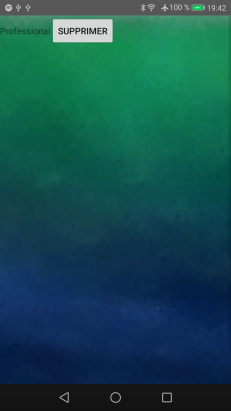
\includegraphics[scale=0.7]{images/list-users-page.png}
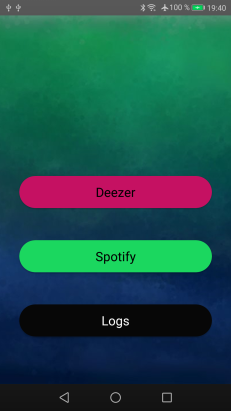
\includegraphics[scale=0.7]{images/login-page.png}
\\
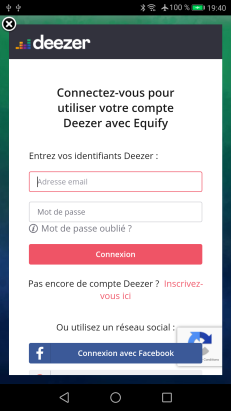
\includegraphics[scale=0.7]{images/deezer-login.png}
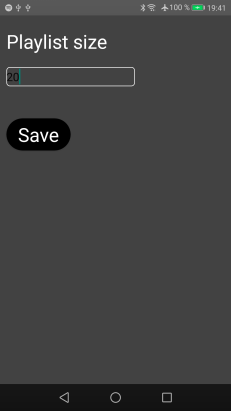
\includegraphics[scale=0.7]{images/setting-page.png}
\\
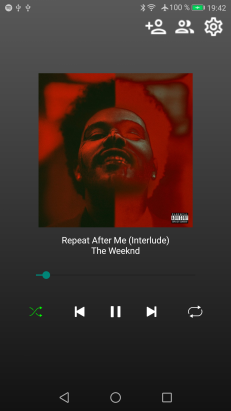
\includegraphics[scale=0.7]{images/media-player-page.png}

\subsection{Illustrations par rapport aux différents besoins énoncés}
 
 \subsubsection{Diagramme des fonctionnalités de l'application}
 
 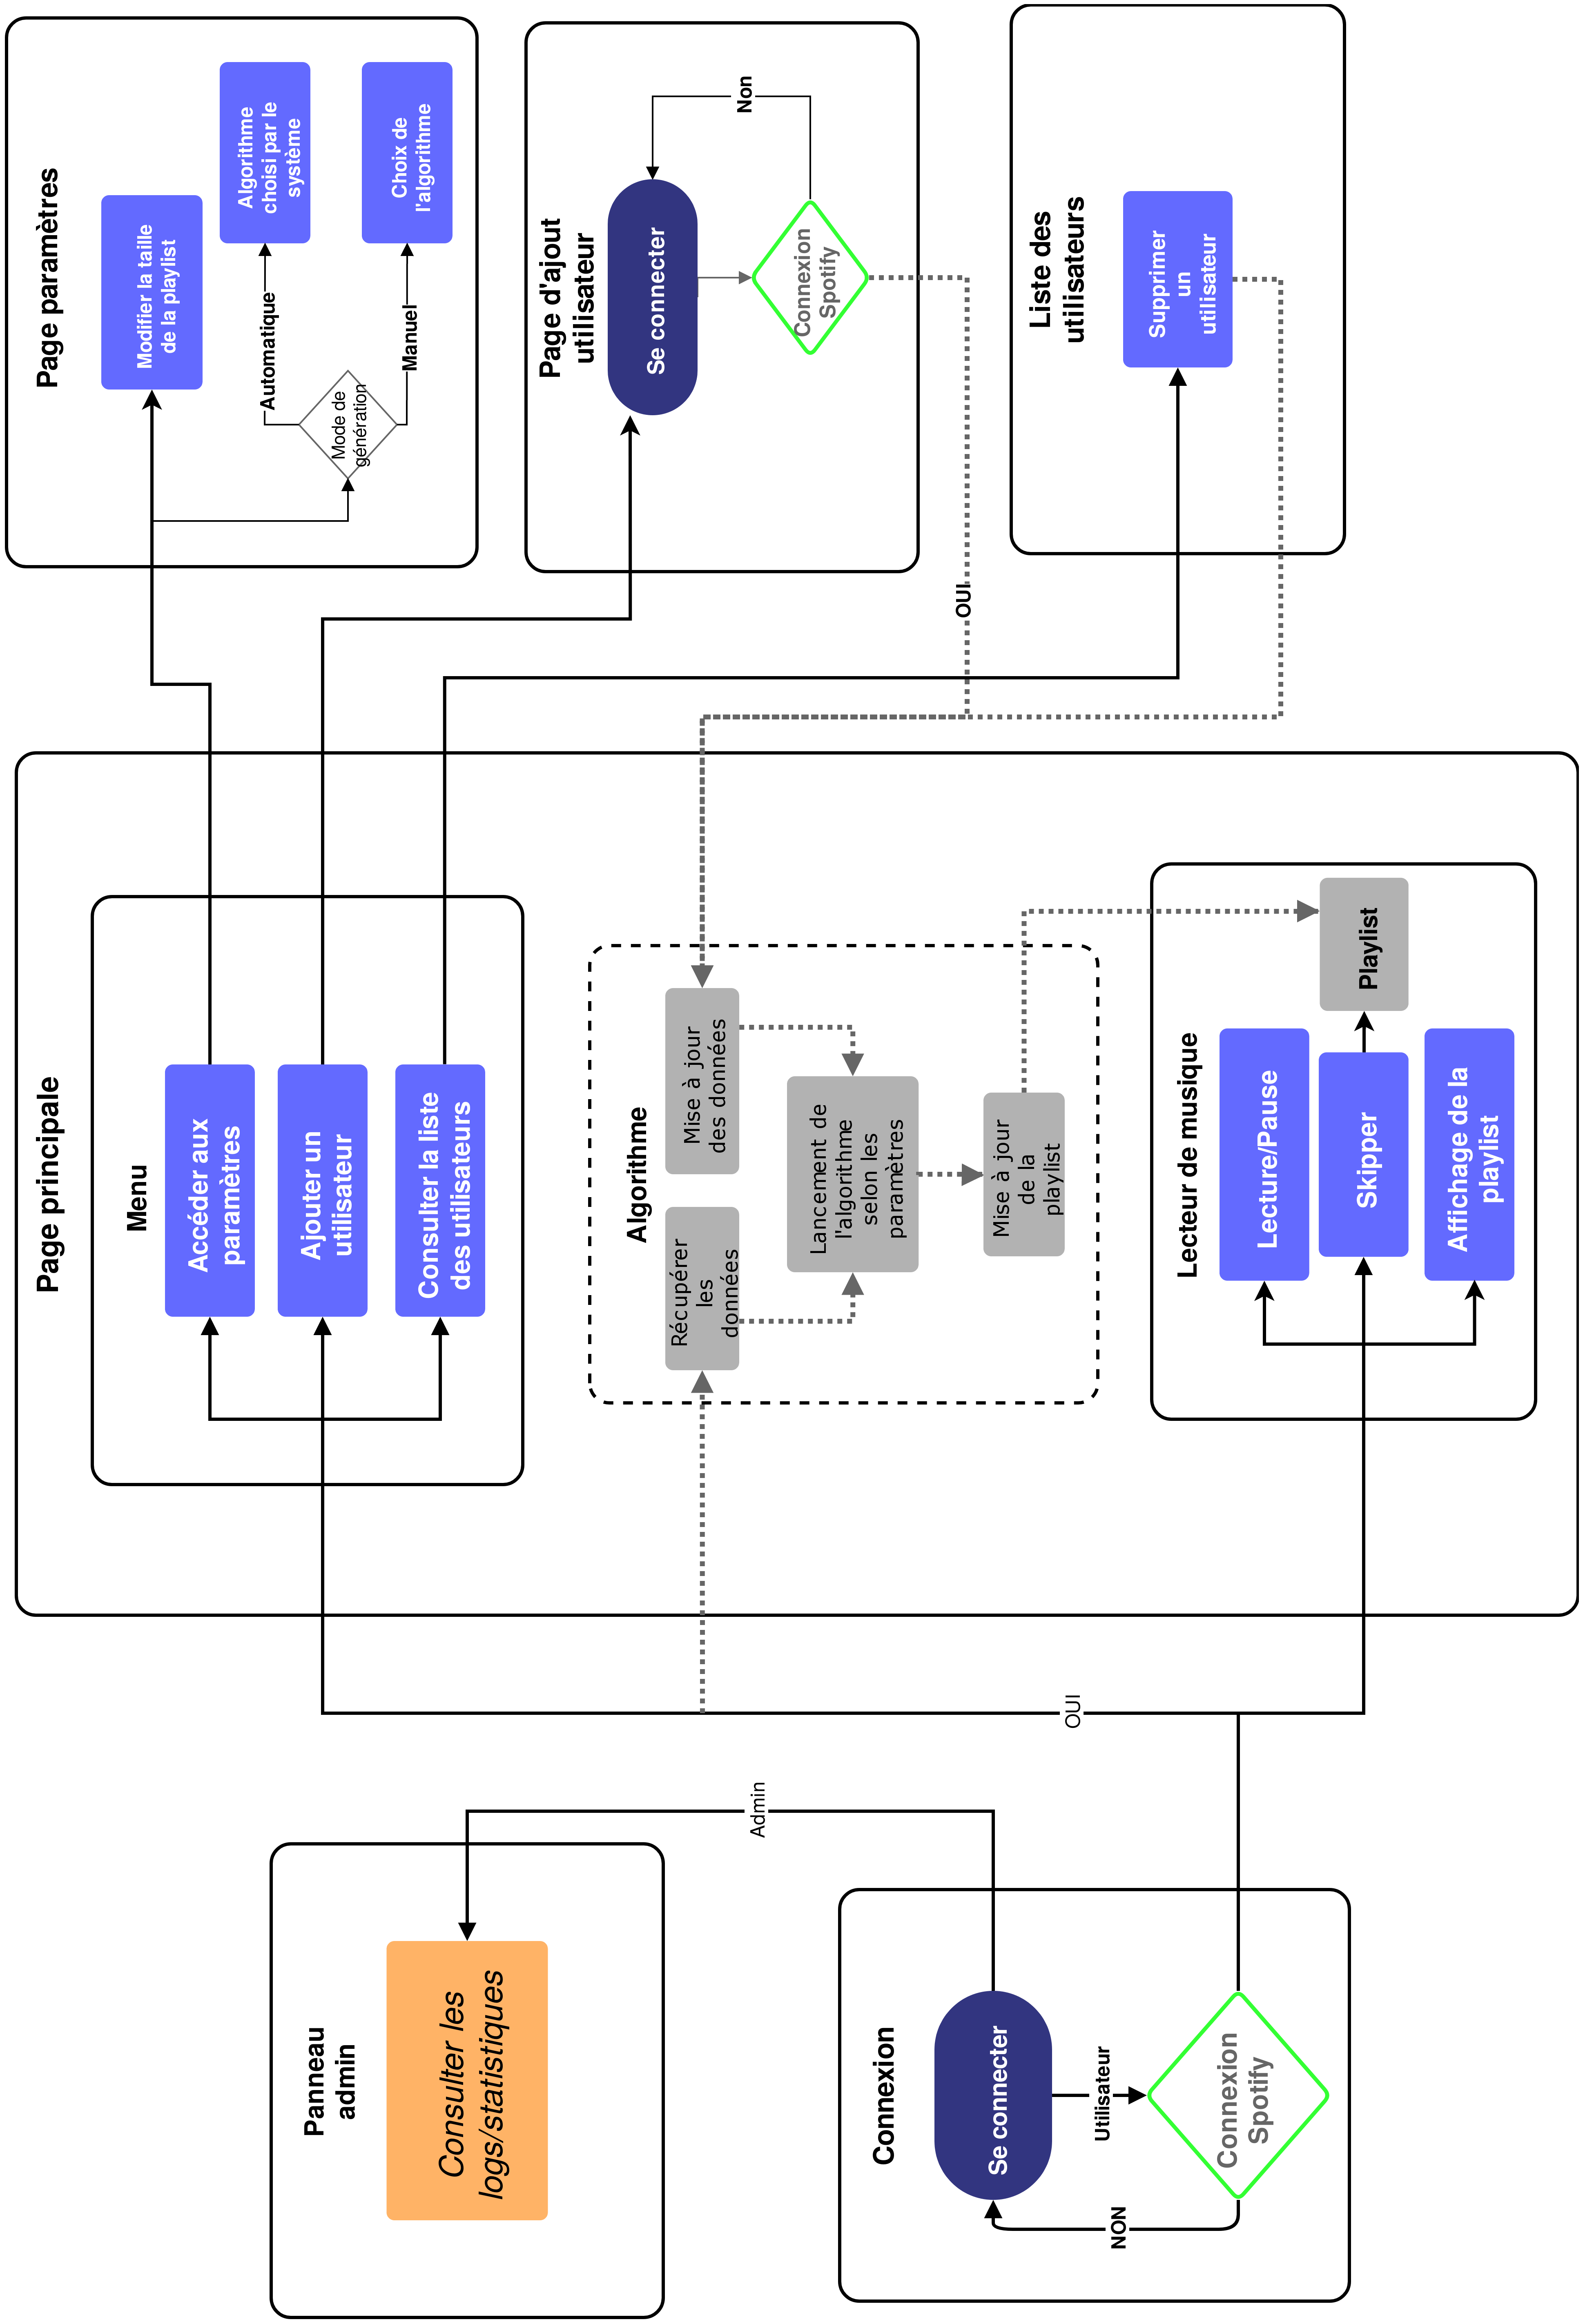
\includegraphics[scale=0.11]{images/schema_fonc.png}
 
 \subsubsection{Scénario d'utilisation}
 
  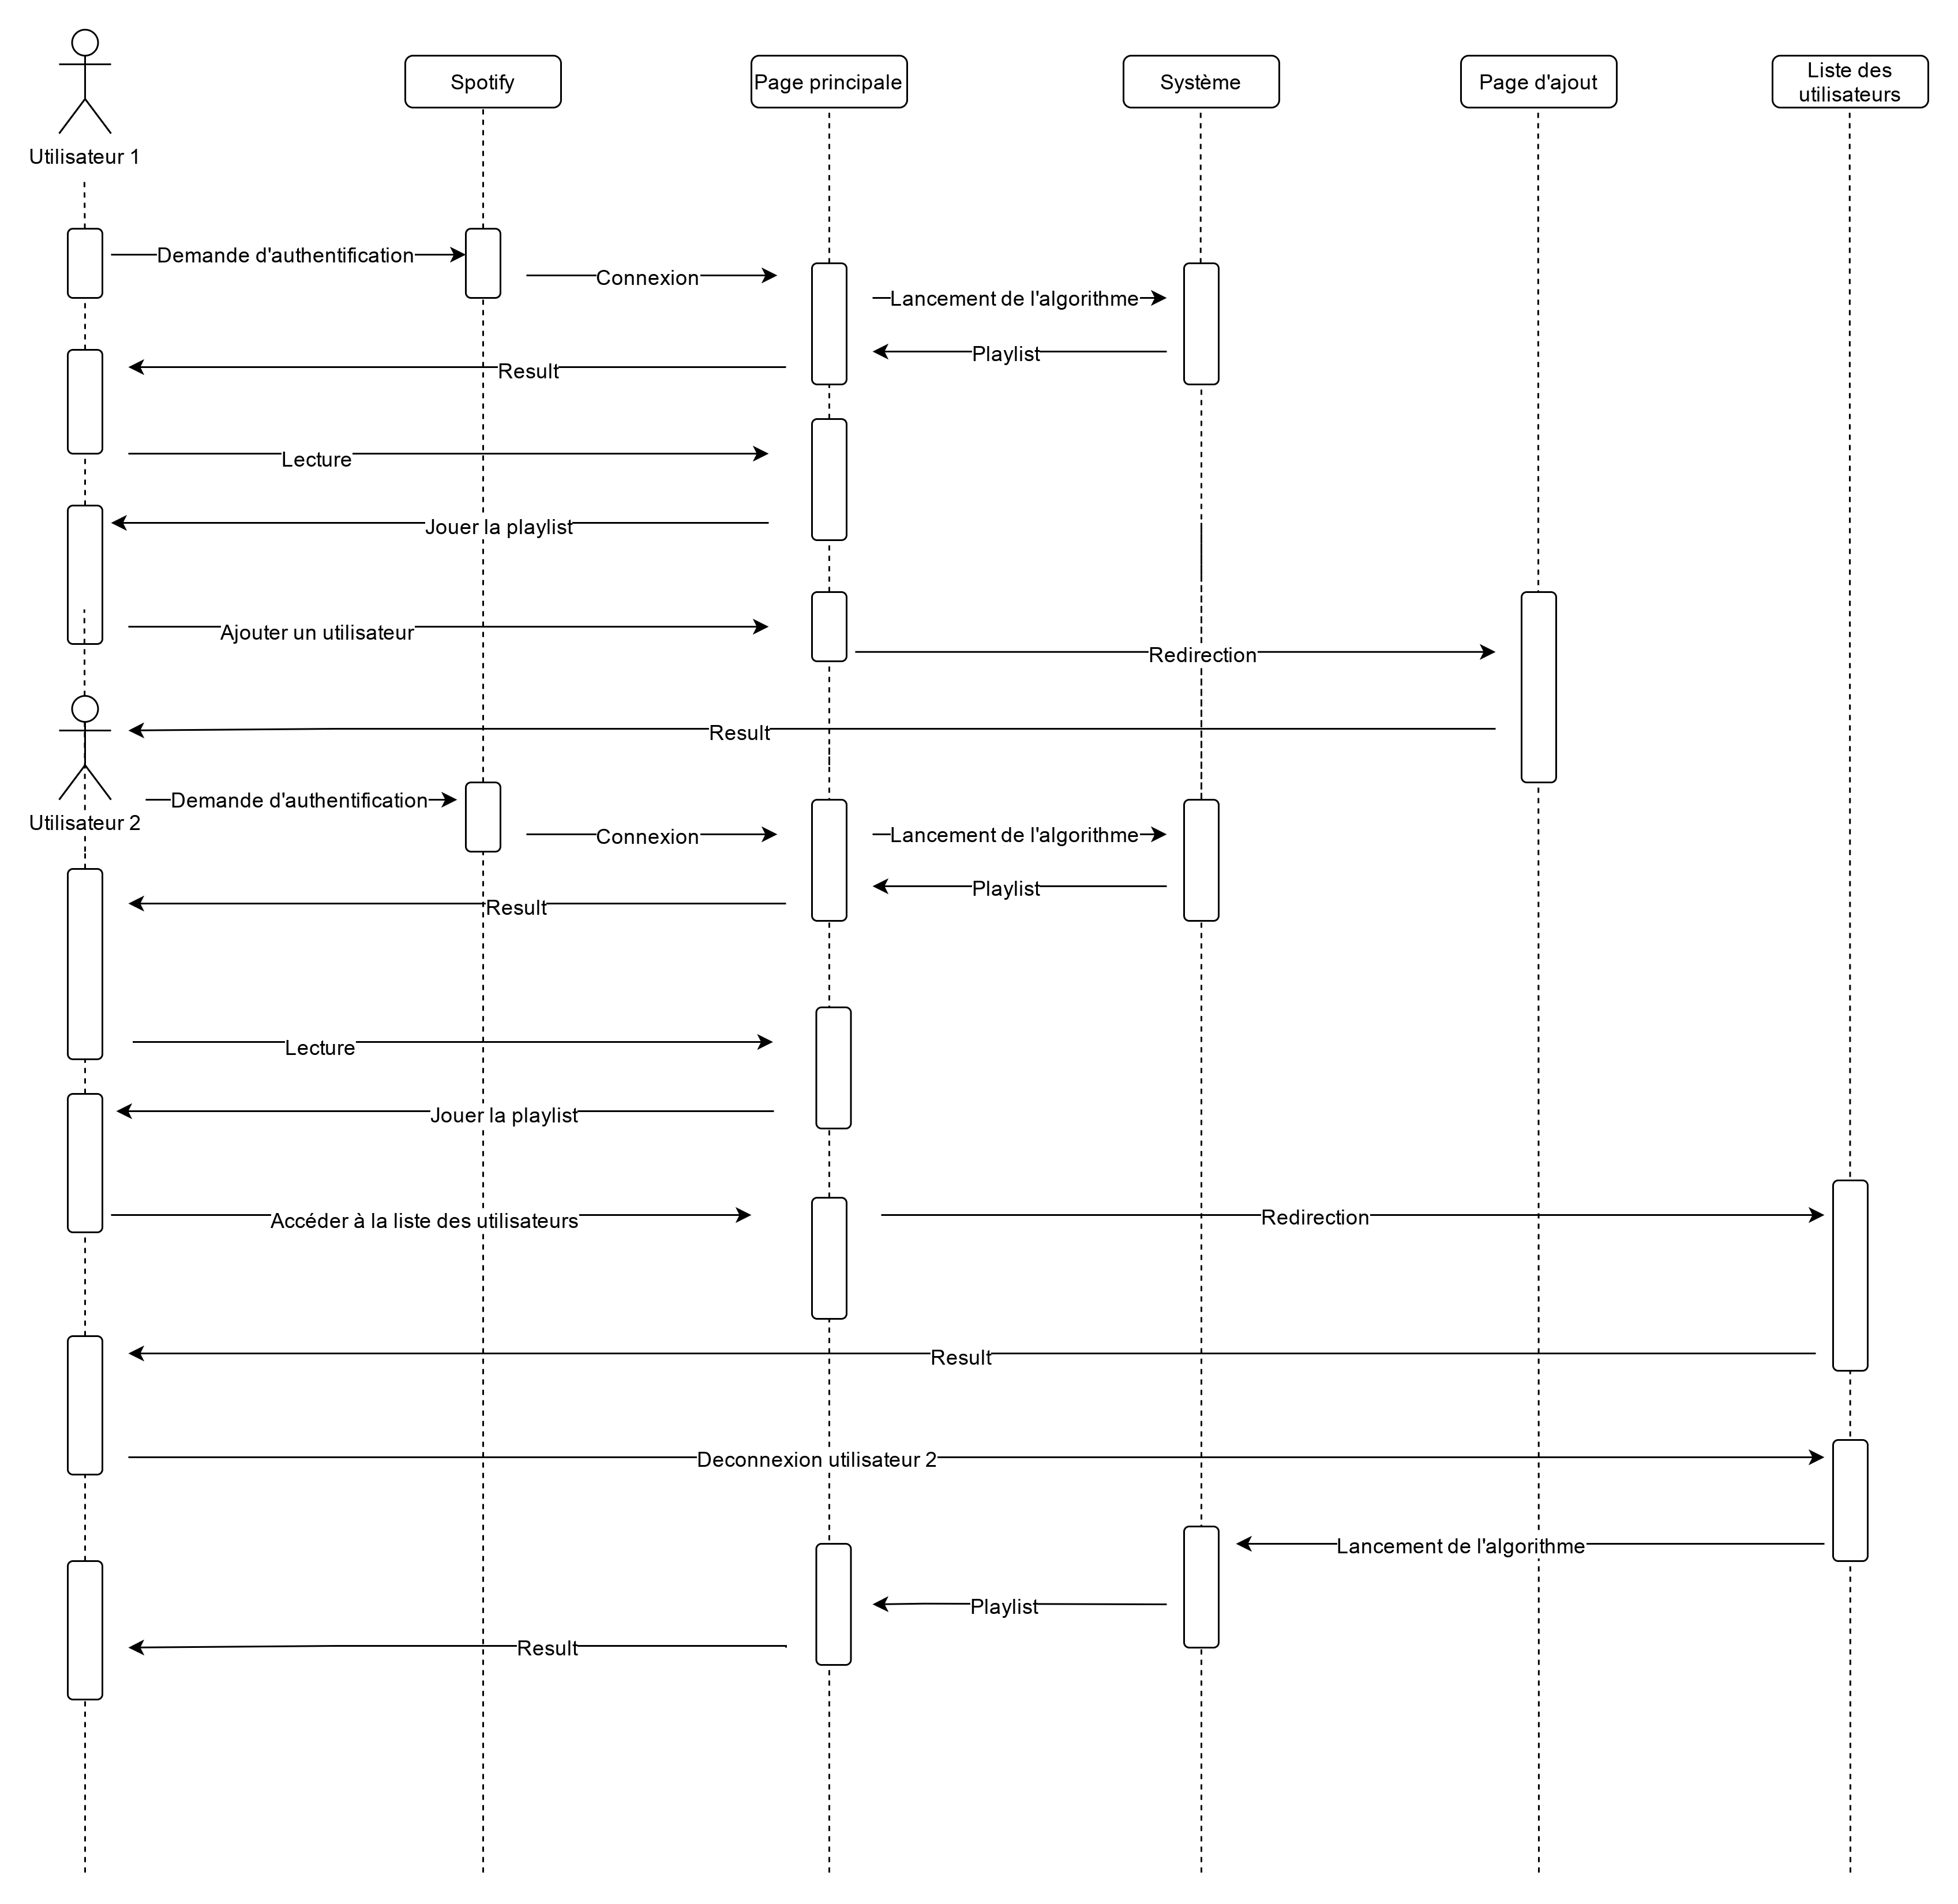
\includegraphics[scale=0.15]{images/scenar_user.png}
  
  \subsubsection{Diagramme de cas d'utilisation UML}
  
  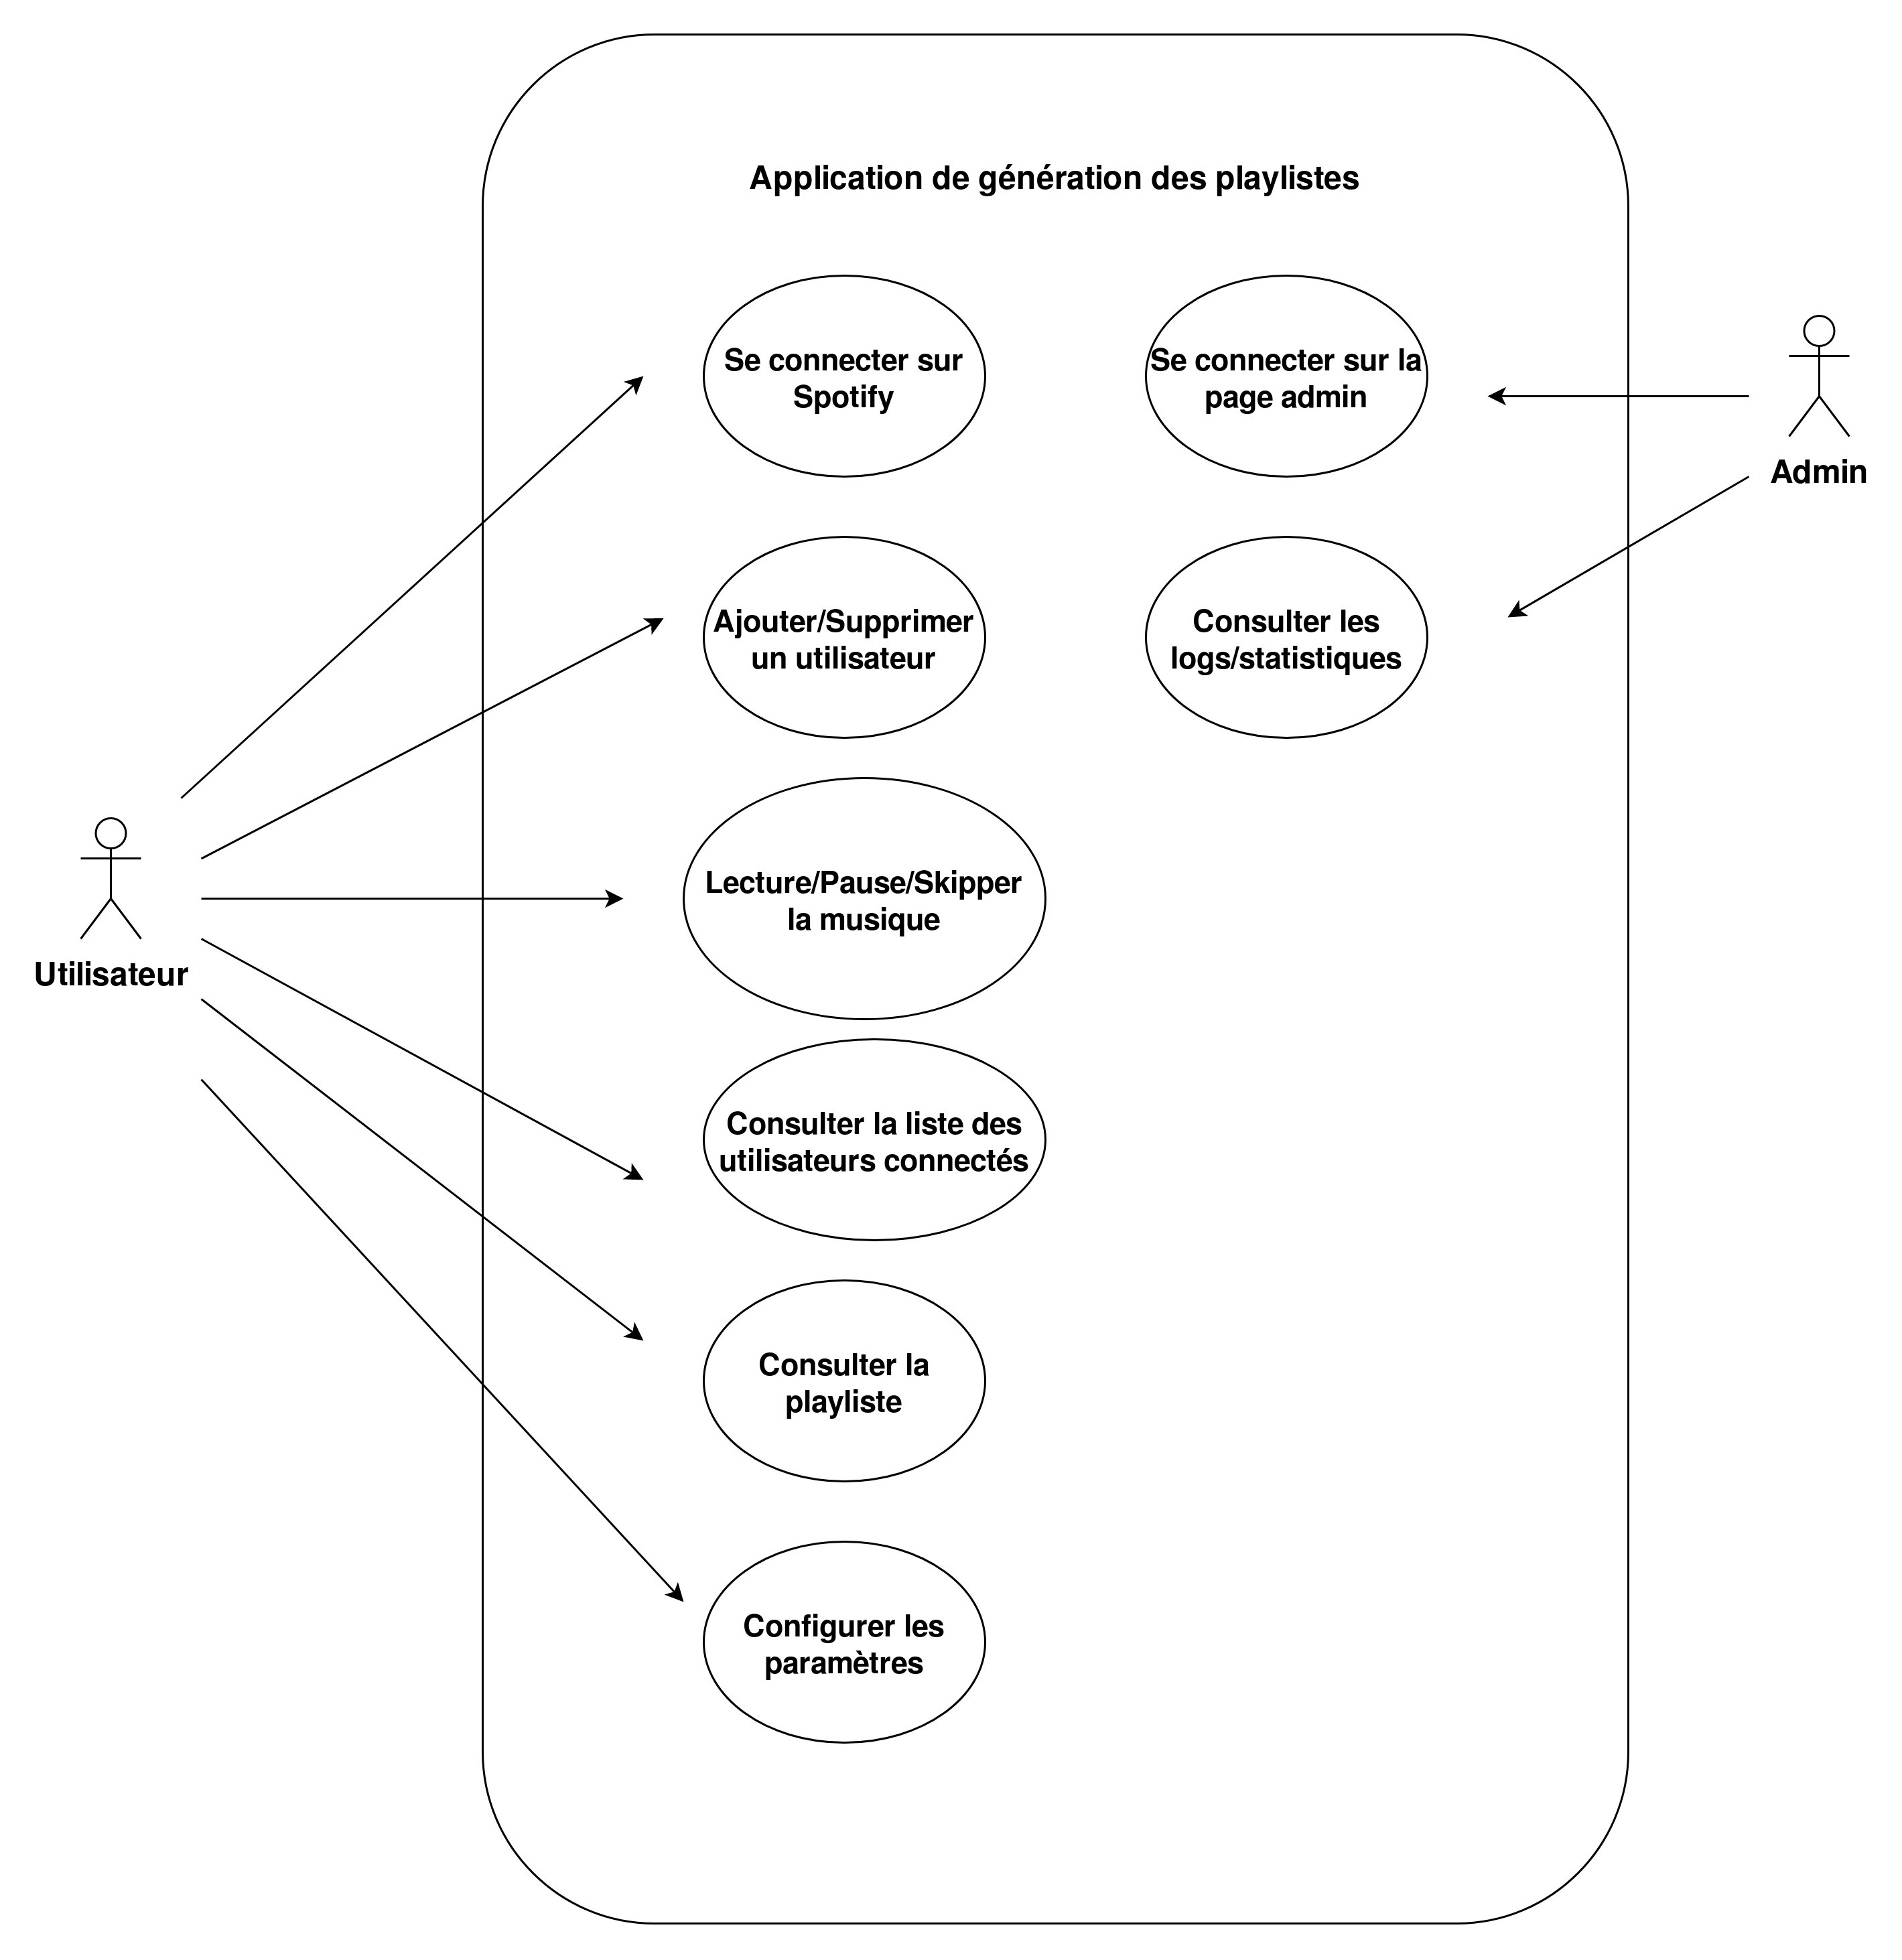
\includegraphics[scale=0.17]{images/cas_dutilisation.png}
  
 \subsubsection{Diagramme de faisabilité par rapport à la récupération des données}
   
   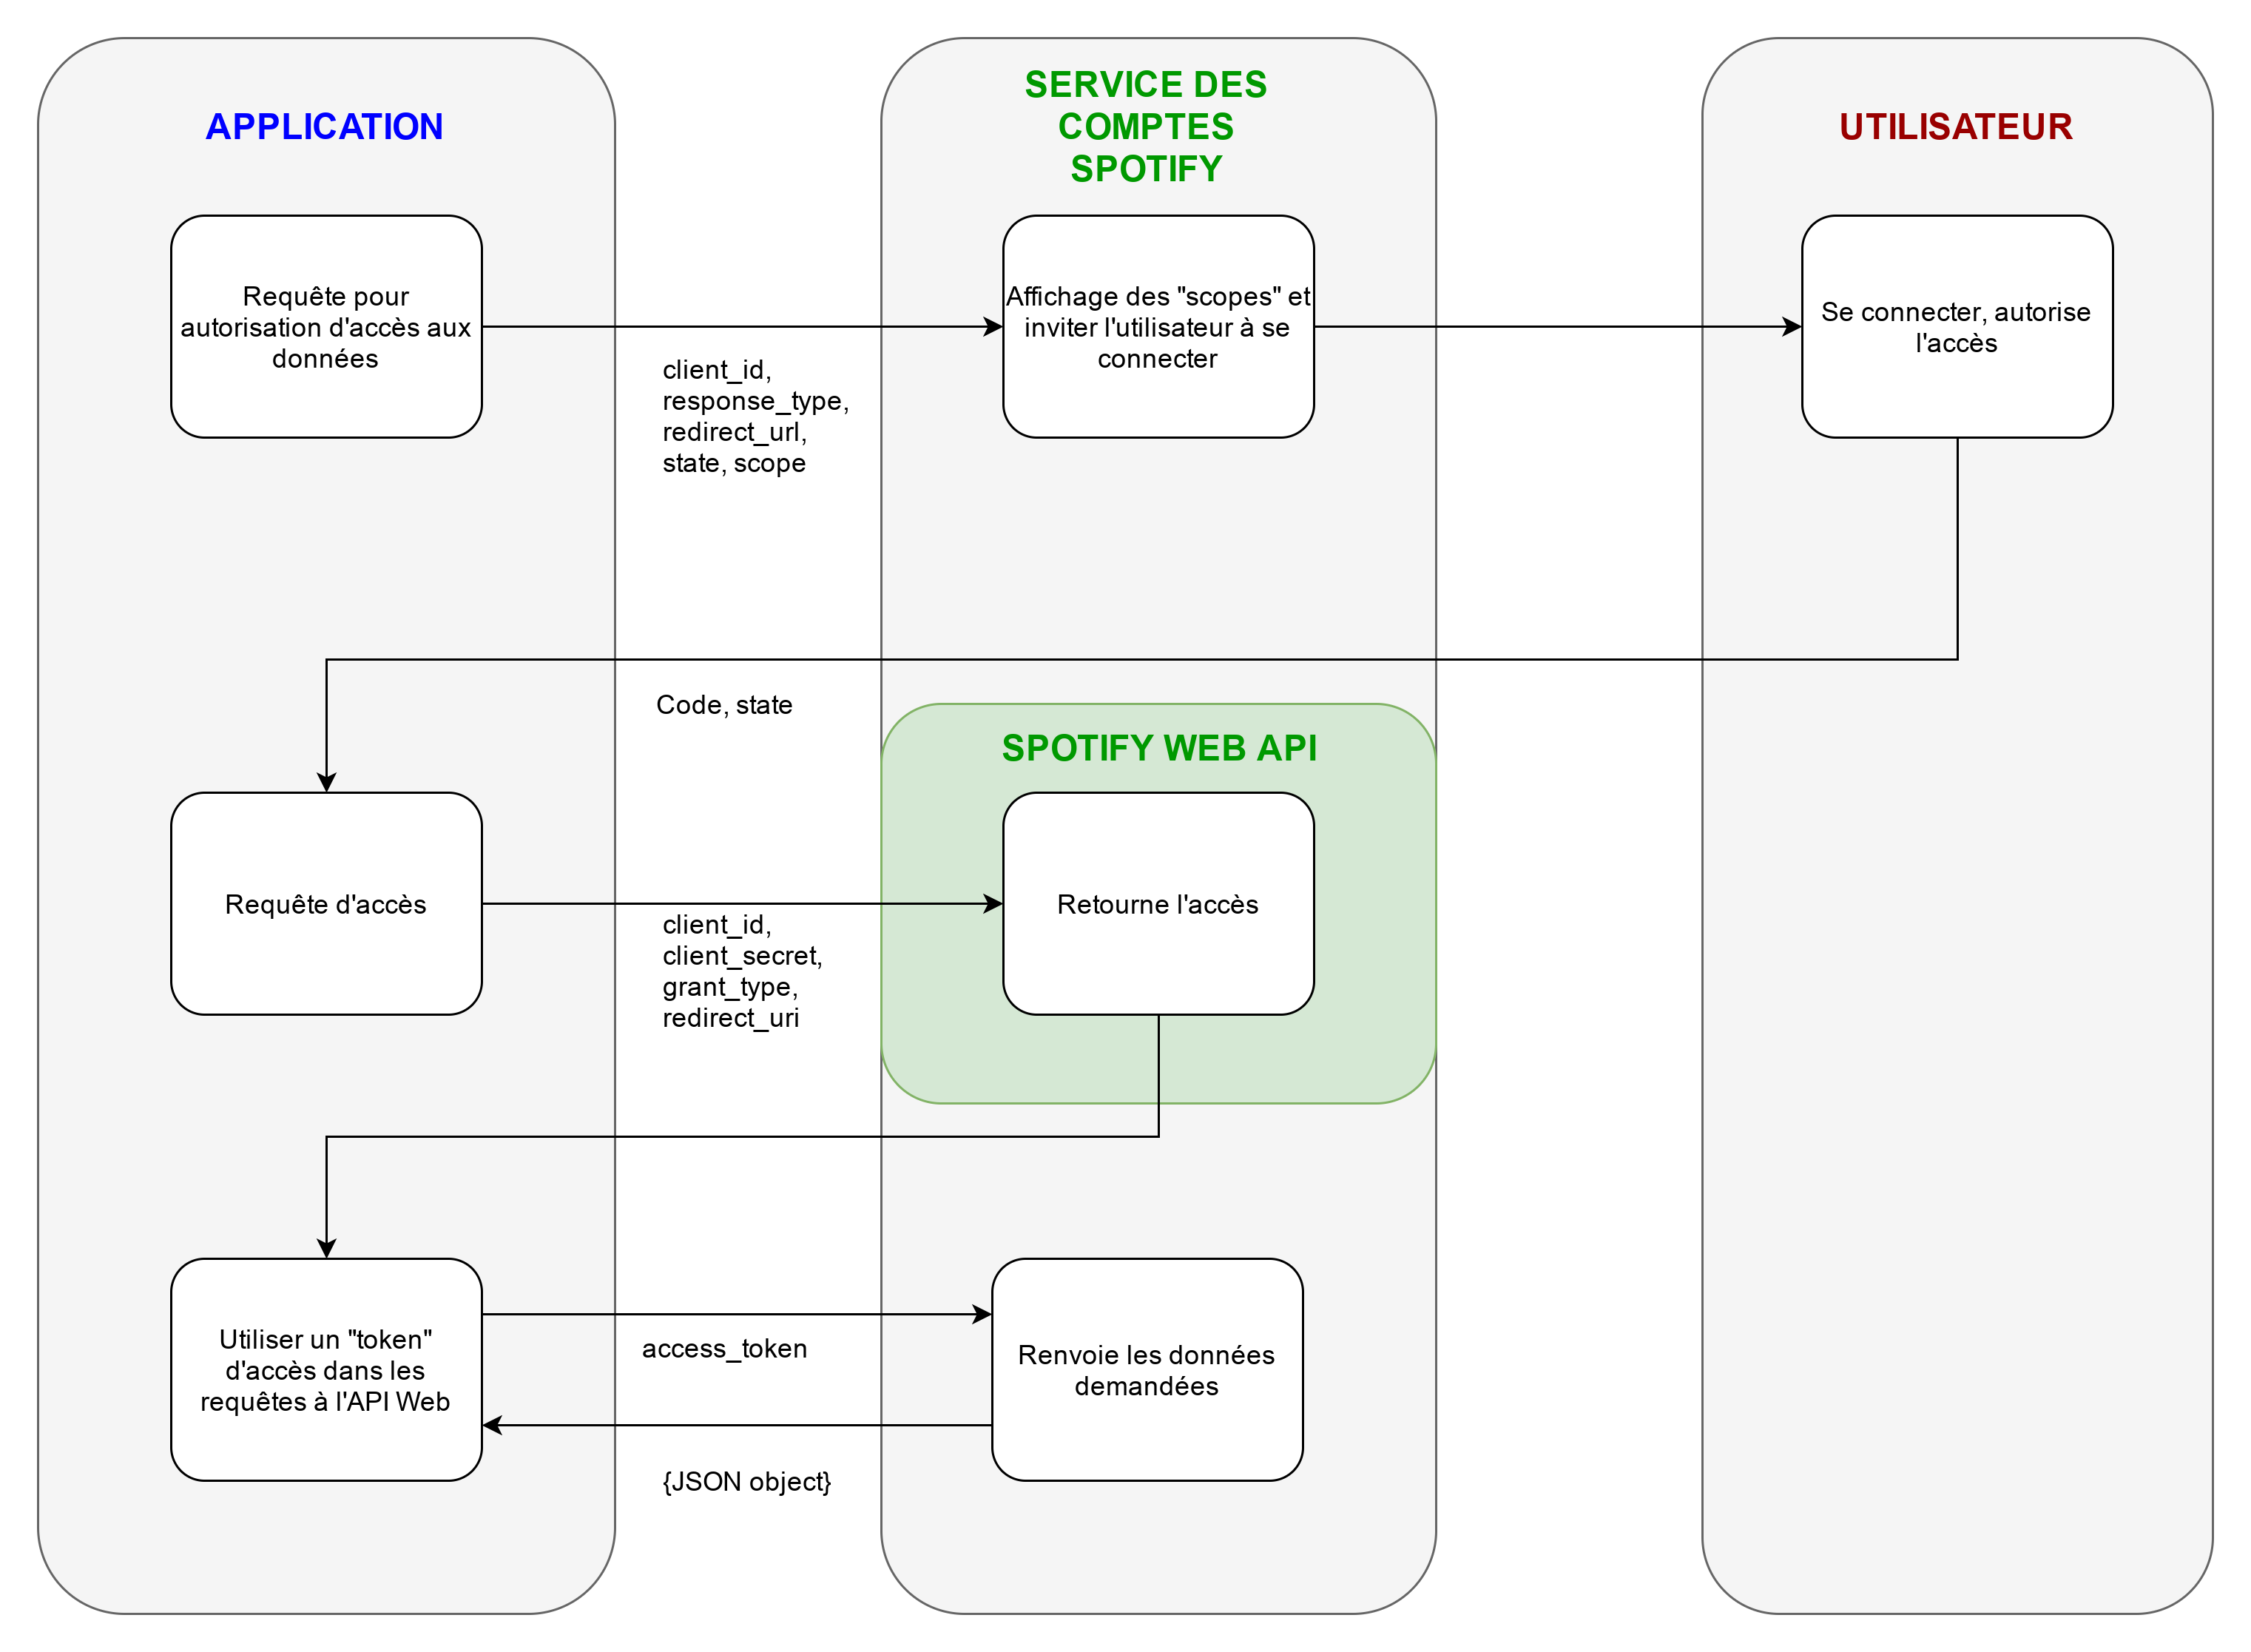
\includegraphics[scale=0.17]{images/schema_faisa_1.png}
   
   \newpage
   
 \subsubsection{Screens sur la possibilité de récupérer les données}
 
    Afin de démontrer la faisabilité du projet, nous avons implémenté, en plus du projet principal, une partie de code permettant de récupérer les données Spotify. Nous les affichons ensuite pour démontrer notre propos. Ci-dessous, le premier screen redirigeant vers une authentification sur l'application Spotify.
    \\
    \\
 
    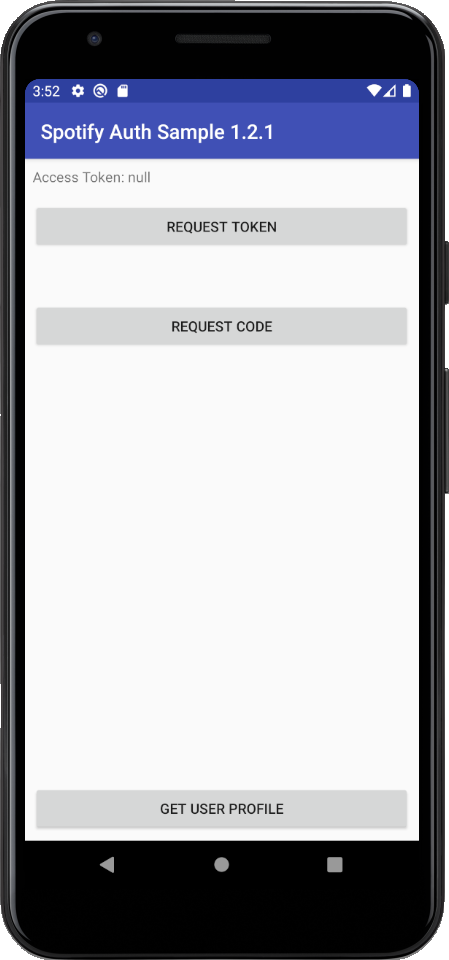
\includegraphics[scale=0.5]{images/recupinfos.png}
    
    \newpage
    
    Après la redirection sur la page d'authentification Spotify (ou Deezer), il est nécessaire que l'utilisateur entre son mail et son mot de passe. Ces données ne relèvent pas de notre application, puisque c'est bien grâce à l'API que l'authentification a lieu. En terme de sécurité, c'est donc la plateforme de streaming qui s'occupe de bien vérifier l'authentification de l'utilisateur, et de s'occuper du chiffrement des données envoyées. \cite{Auth}
    \\
    \\
    
    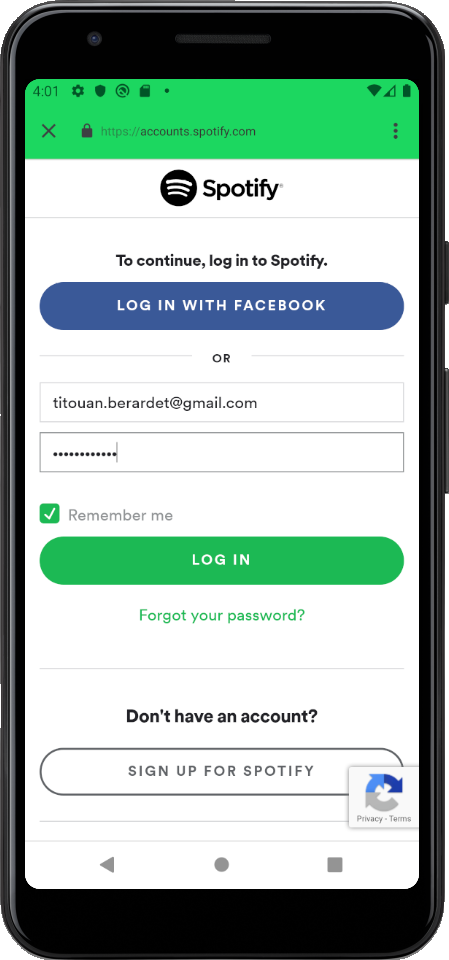
\includegraphics[scale=0.5]{images/authentification_exemple.png}
    
    \newpage
    
    Après l'authentification, la plateforme d'écoute demande à l'utilisateur s'il autorise l'application à accéder à ses données, en plus d'accéder à ses dernières activités.
    \\
    \\
    
    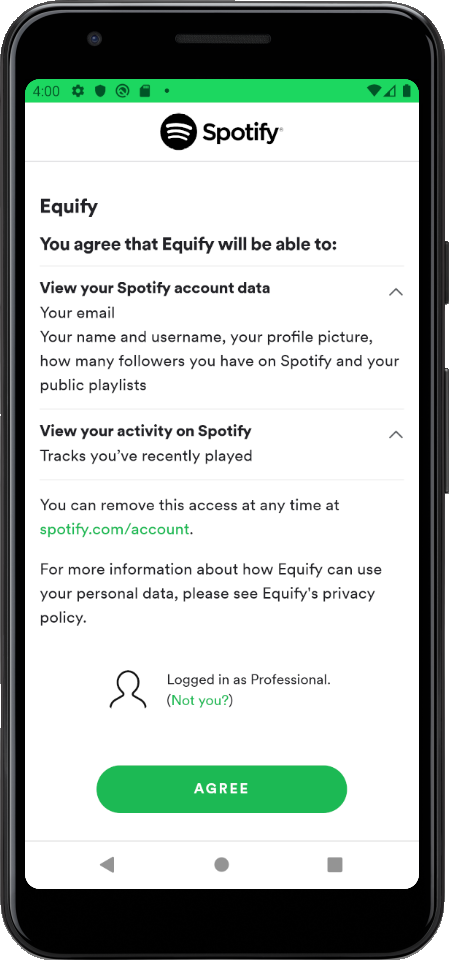
\includegraphics[scale=0.5]{images/accord_spotify.png}
    
    \newpage
    
    A partir de là, nous faisons des requêtes de type GET par l'intermédiaire de l'API Spotify, afin de récupérer un fichier JSON contenant les premières informations permettant de faire tourner le reste de l'application, soit l'ID et le token de l'utilisateur. Nous les affichons sur l'image ci-dessous, afin d'attester de la véracité de nos propos.
    \\
    \\
    
    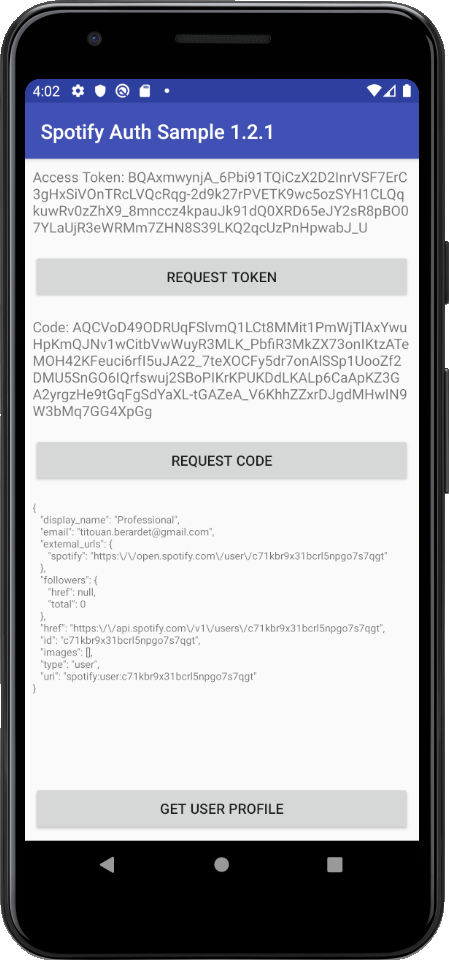
\includegraphics[scale=0.5]{images/informations.png}
    
\subsection{Diagramme de Gantt}


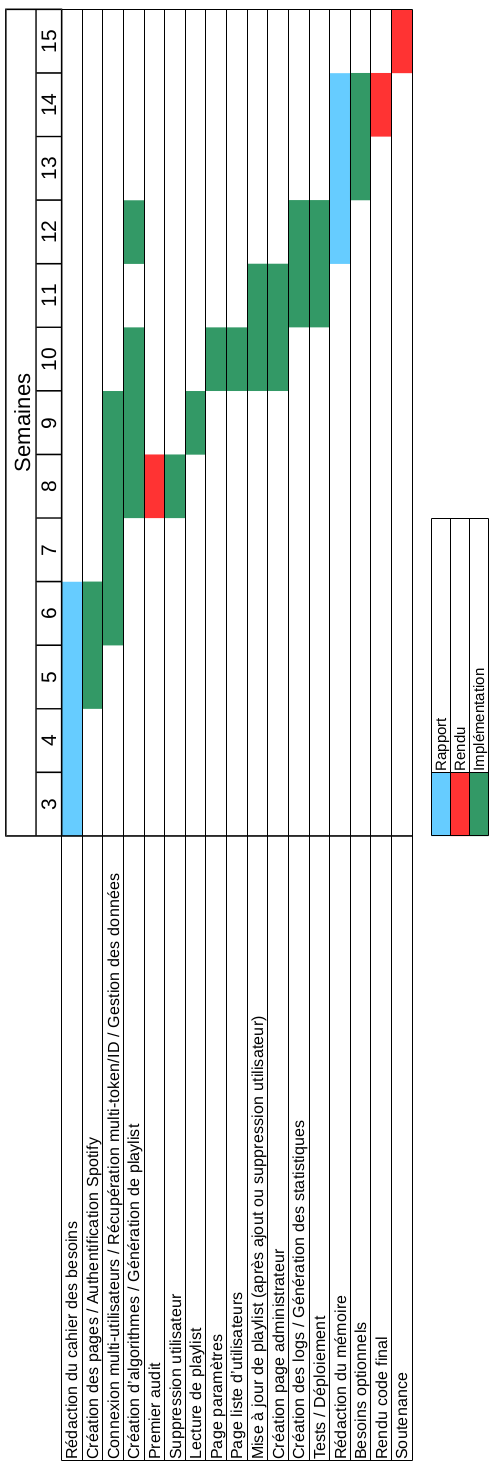
\includegraphics[scale=0.45]{images/gantt.png}


\bibliography{biblio}

\end{document}